\documentclass[../electromagnetism.tex]{subfiles}
\begin{document}
\section{Principle of Relativity}
The principle of relativity states a quite simple but deep affirmation: \emph{All interaction propagate at a constant speed independent from the chosen frame of reference}. This speed is usually denoted as $c$ and it's informally known as the speed of light, which has the following value (in SI units)
\begin{equation}
	c=2.998\times10^8\ \mathrm{m/s}
	\label{eq:clight}
\end{equation}
In the part on classical mechanics we always intended between the lines that all interactions are instantaneous and therefore we'd have $c\to\infty$ formally. This can be interpreted as taking classical mechanics as an approximation of Einstein's relativity for which $v/c<<1$, which is the case for our really slow classical particles.\\
Note that this constant speed of propagation precludes that time isn't universal, and it is frame dependent. In order to understand this it's useful to get two coordinate frames $K$ and $\tilde{K}$, where one is moving with respect to the other with a constant speed $V$.\\
Suppose now that a point $A$ emits a signal towards two other points $B$ and $C$ %doesn't matter
%
\begin{figure}[H]
	\centering
	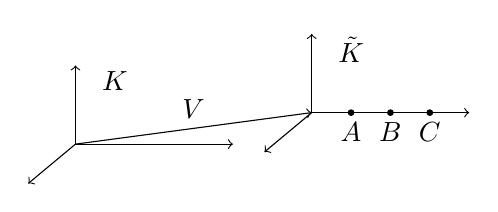
\begin{tikzpicture}
		\draw[->] (0,0) -- (0,1);
		\draw[->] (0,0) -- (2,0);
		\draw[->] (0,0) -- (-0.6,-0.5);
		\node at (0.5,0.8) {$K$};
		\draw[->] (3,0.4) -- (5,0.4);
		\draw[->] (3,0.4) -- (3,1.4);
		\draw[->] (3,0.4) -- (2.4,-0.1);
		\node at (3.5,1.2) {$\tilde{K}$};
		\draw[->] (0,0) -- (3,0.4);
		\node[above] at (1.5,0.2) {$V$};
		\draw[fill=black] (3.5,0.4) circle (1pt);
		\draw[fill=black] (4,0.4) circle (1pt);
		\draw[fill=black] (4.5,0.4) circle (1pt);
		\node[below] at (3.5,0.4) {$A$};
		\node[below] at (4,0.4) {$B$};
		\node[below] at (4.5,0.4) {$C$};
	\end{tikzpicture}
	\label{fig:srframestime}
	\caption{The two frames $K$ and $\tilde{K}$}
\end{figure}
In the frame $\tilde{K}$, where $A$ is at rest, we see that the signal reaches both points at the same time, but the same CANNOT be true for the other system, since the relativity principle would be violated. Thinking in a different way, suppose that you're standing at the origin of the $K$ system. If the velocity of the signal is constant in all reference frames we can for sure say that it's so where we're standing, therefore we end up seeing $B$ moving towards the signal and $C$ moving away from it, both with speed $V$. In this system we therefore must see a delay in when the two points receive such signal.\\
Although counterintuitive we're experimentally more than sure that this is actually a better approximation of nature than our beloved Newtonian mechanics.
\section{Spacetime}
Since time it's not anymore an universal thing and behaves itself as a coordinate, we can now think of our universe as a $4D$ manifold with time as a new coordinate. This is known as \emph{Minkowsky Spacetime} or in short as \emph{Spacetime}. This new definition follows:
\begin{dfn}[Event]
	Given a spacetime with coordinates $(ct,x,y,z)$ with $c$ the speed of light, we define a point in spacetime as an \emph{event} in such.\\
	Since time only ``flows'' one way, we have that for every particle corresponds a wordline which connects all the events pertaining to such. Note that events are also known as \emph{universe points}
\end{dfn}
Given the principle of relativity one might also ask rightfully how to formulate mathematically all of this, bringing out some invariants that might help with further derivations. Take again the previous system and call $l$ the distance traveled by the signal after being emitted from $A$. Calling $t_1$ and $t_2$ the emission time and the arrival time respectively, we have that for obvious reasons
\begin{equation}
	l=c(t_1-t_2)
	\label{eq:ltrd1}
\end{equation}
But, we can also write as follows
\begin{equation}
	l=\sqrt{(x_2-x_1)^2+(y_2-y_1)^2+(z_2-z_1)^2}
	\label{eq:ltrd2}
\end{equation}
With $(x_1,y_1,z_1)$ being the departure coordinates and $(x_2,y_2,z_2)$ the arrival coordinates in $K$
In $\tilde{K}$, analogously we have
\begin{equation}
	\begin{aligned}
		\tilde{l}&=c(\tilde{t}_2-\tilde{t}_1)\\
		\tilde{l}&=\sqrt{(\tilde{x}_2-\tilde{x}_1)^2+(\tilde{y}_2-\tilde{y}_1)^2+(\tilde{z}_2-\tilde{z}_1)^2}
	\end{aligned}
	\label{eq:ltrdtil}
\end{equation}
Tying up both equations we end with the following result
\begin{equation}
	\left\{\begin{aligned}
		c^2(t_2-t_1)^2-(x_2-x_1)^2-(y_2-y_1)^2-(z_2-z_1)^2&=0\\
		c^2(\tilde{t}_2-\tilde{t}_1)^2-(\tilde{x}_2-\tilde{x}_1)^2+(\tilde{y}_2-\tilde{y}_1)^2+(\tilde{z}_2-\tilde{z}_1)^2&=0
	\end{aligned}\right.
	\label{eq:interval1}
\end{equation}
In ``layman'' words this basically means, that the following quantity
\begin{equation}
	s^2_{12}=c^2(t_2-t_1)^2-(x_2-x_1)^2-(y_2-y_1)^2-(z_2-z_1)^2
	\label{eq:intervalsr}
\end{equation}
Called, \emph{interval}, is a \emph{relativistic invariant}, and therefore invariant with respect to changes of coordinate frames in the context of special relativity.\\
From \eqref{eq:interval1} we have that if the two points are infinitesimally close to eachother we can define the infinitesimal interval as
\begin{equation}
	\dd s^2=c^2\dd t-\dd x^2-\dd y^2-\dd z^2
	\label{eq:diffint}
\end{equation}
The invariance of such differential quantity is easy to show considering the previous case we stated where $\dd s=\dd\tilde{s}=0$ we have, using basic intuition that
\begin{equation}
	\dd s^2=a(V)\dd\tilde{s}^2
	\label{eq:invarproof}
\end{equation}
Where $a(V)$ is a function of the relative velocity between the two considered frames. It cannot depend on direction due to the isotropy of space.\\
Consider now three inertial reference frames $K,K_1,K_2$, and let $V_1,V_2$ be the velocities of the frames $K_1,K_2$. We can therefore say, using \eqref{eq:invarproof} that
\begin{equation}
	\begin{aligned}
		\dd s^2&=a(V_1)\dd s^2_1=a(V_2)\dd s^2_2\\
		\dd s^2_1&=a(V_{12})\dd s^2_2
	\end{aligned}
	\label{eq:invarproof2}
\end{equation}
Where we defined the velocity between $K_1,K_2$ as $V_{12}$. Rewriting the equation we have
\begin{equation*}
	\dd s^2=a(V_1)a(V_{12})\dd s^2_2=a(V_2)\dd s^2_2
\end{equation*}
Equating the coefficients of the differential $\dd s_2$, we have
\begin{equation}
	a(V_{12})=\frac{a(V_2)}{a(V_1)}
	\label{eq:v12lreq}
\end{equation}
The previous equation then might be true if and only if $a(V_{12})$ depends only on the angle between the velocities $V_1,V_2$. This cannot be true due to the isotropy of spacetime, as we stated for the previous problem, and therefore $a(V)$ might only be a constant function. Taking $a(V_{12})=1$ for consistency between frames of reference, we have finally demonstrated that the differential spacetime interval is invariant
\begin{equation}
	\dd s=\dd\tilde{s}
	\label{eq:infsinv}
\end{equation}
This definition of $\dd s$ gives rise to three kinds of intervals:
\begin{enumerate}
\item \emph{Spacelike intervals} if $s_{12}^2<0$
\item \emph{Timelike intervals} if $s_{12}^2>0$
\item \emph{Light-like intervals} if $s_{12}^2=0$
\end{enumerate}
These three distinctions let us answer two previously impossible questions: is it possible to find a reference frame where two events happen at the same time or at the same place in our three-dimensional perception?. The answer is surprisingly \textit{yes}. It depends on the kind of the interval between the two points.\\
Let's work with the first assumption, taken two events in spacetime $E_1,E_2$, defined $t_{12}=t_2-t_1$ and $l_{12}$ as our usual 3D distance between the events, we have
\begin{equation*}
	s_{12}^2=c^2t_{12}^2-l^2_{12}
\end{equation*}
Let's now search a system where $l_{12}'=0$. In order to have this, using that $s_{12}=s_{12}'$ we have
\begin{equation*}
	s_{12}=c^2t_{12}-l^2_{12}=c^2t^{'2}_{12}=s_{12}^{'2}>0
\end{equation*}
I.e. the spacetime interval between the frame of reference at rest with respect to the two events and the new unknown frame of reference is timelike.\\
Analogously, if we wanted to find a new system where the two events happen at the same time, we might have set $t_{12}'=0$, therefore getting
\begin{equation}
	s_{12}=c^2t_{12}-l^2_{12}=l^{'2}_{12}=s_{12}^{'2}<0
	\label{eq:spacelike}
\end{equation}
\subsection{Spacetime Diagrams}
The idea of spacetime and absoluteness of the velocity of interactions can be described well by a 2D spacetime diagram. Taken an origin for our system of coordinates $(ct,x)$ we have that, considering $v$ as the slope of a constant wordline, that $\abs{v}<c$.
\begin{figure}[H]
	\centering
	\begin{tikzpicture}
		\draw[->] (0,-4) -- (0,4) node[right] {$ct$};
		\draw[->] (-3,0) -- (3,0) node[below] {$x$};
		\draw (-3,-3) -- (3,3) node[above] {$v=c$};
		\draw (-3,3) -- (3,-3) node[below] {$v=-c$};
		\node at (2.5,1) {Unreachable};
		\node at (-2.5,-1) {Unreachable};
		\node at (-1.3,-2.5) {Past};
		\node at (1.3,2.5) {Future};
	\end{tikzpicture}
	\caption{Simple spacetime diagram. Note how all the events beyond the asymptote (or \emph{horizon}) $v=\pm c$ are inaccessible from $0$}
	\label{fig:stdiag}
\end{figure}
Thought in higher dimensions we have that all the past and future of an event are enclosed inside a cone bordered by our horizon $\abs{v}=c$ which separates physical impossibilities from the actual physical past and future of what we're considering.\\
Note that if $v=\pm c$ we must have $x=\pm ct$, giving us a spacelike interval for our diagram.\\
Considering instead past and future it's also easy to see that the past is always spacelike, since $c^2t^2-x^2<0$, and that the future is always timelike. Note also that past and future must be absolute
\section{Proper Time}
Since time is not a relativistic invariant, we need to search for a good substitute of it. Given a clock fixed at the origin of some inertial frame $K'$. After some time $\dd t$, the clock has moved (in our system) by the following quantity
\begin{equation*}
	\sqrt{\dd x^2+\dd y^2+\dd z^2}
\end{equation*}
By definition, in $K'$ this clock is at rest, therefore we have
\begin{equation*}
	\dd x'=\dd y'=\dd z'=0
\end{equation*}
Imposing the invariance of intervals we have that
\begin{equation}
	\dd s^2=c^2\dd t^2-\dd x^2-\dd y^2-\dd z^2=c^2\dd t^{'2}
	\label{eq:invclock}
\end{equation}
Therefore, it must be true that
\begin{equation}
	\dd t'=\dd t\sqrt{1-\frac{\dd x^2+\dd y^2+\dd z^2}{c^2\dd t^2}}
	\label{eq:proptime}
\end{equation}
This is the expression for the passing of time in the system where the clock is at rest, and it's called the \emph{proper time} of the clock, usually indicated with $\tau$. Writing the sum of differentials as $\dd r^2$ and using the definition of $v^2$, we have that
\begin{equation}
	\dd\tau=\dd t\sqrt{1-\frac{v^2}{c^2}}=\frac{\dd s}{c}
	\label{eq:diffprpot}
\end{equation}
Integrating and using the fundamental theorem of calculus, we have that a given time interval will be ``felt'' differently by the clock, where
\begin{equation}
	\Delta\tau=\int_{\tau_1}^{\tau_2}\sqrt{1-\frac{v^2}{c^2}}\dd t<\Delta t
	\label{eq:proptimeint}
\end{equation}
This tells us that a moving clock will tick slower than a clock at rest (note also on how this definition depends directly on the chosen frame).\\
This difference of measured time is known as \emph{time dilation}.
\section{Formalization of the Principle of Relativity}
All of what we found before can be crammed into the most fundamental element of relativity: coordinate transformations.\\
Consider two reference frames $K,\ (ct,x,y,z)$ and $K',\ (ct,x,y,z)$. Mathematically, what we call interval is the usual 4D distance in a seminegative definite metric, and due to its invariance we must have that all coordinate transformations between these two systems must be rototraslations (isometries). Translations can be immediately ignored since they only move the origin of the system, and therefore we choose our faithful rotations in order to find these coordinate transformation laws.\\
All the possible rotations are between the planes $xy,xz,yz$ and $tx,ty,tz$. All rotations $xy,xz,yz$ are our usual 3D rotations and are of no use, therefore we choose the rotations $tx,ty,tz$. Taking $tx$ as the chosen one we have that the spacetime interval is
\begin{equation*}
	s^2=c^2t^2-x^2
\end{equation*}
Therefore, all searched rotations \textit{must preserve} this relationship. The first idea one might have is to look at the symmetry of the system and deduce immediately that such rotation must be hyperbolic in nature. We therefore define the following
\begin{equation}
	\begin{pmatrix}x\\ct\end{pmatrix}=\begin{pmatrix}\cosh\psi&\sinh\psi\\\sinh\psi&\cosh\psi\end{pmatrix}\begin{pmatrix}x'\\ct'\end{pmatrix}
	\label{eq:hyprotm}
\end{equation}
Taking $x'=0$ it all reduces to this single equation
\begin{equation}
	\frac{x}{ct}=\frac{V}{c}=\tanh\psi
	\label{eq:ctransfhyp}
\end{equation}
It's common to indicate such value with the pure number $\beta$, called the \emph{Lorentz Boost}, where
\begin{equation*}
	\beta=\frac{V}{c}
\end{equation*}
%I WILL PUT THE SOLVED EQUATIONS IN THE APPENDIX OR LATER HERE PLEASE DON'T HURT ME
Solving \eqref{eq:ctransfhyp} we have that
\begin{equation}
	\beta=\frac{\sinh\psi}{\sqrt{1+\sinh^2\psi}}=0\implies\sinh^2\psi=\frac{\beta}{\sqrt{1-\beta^2}}
	\label{eq:sinh1}
\end{equation}
And
\begin{equation}
	\cosh^2\psi=1+\sinh^2\psi\implies\cosh\psi=\frac{1}{\sqrt{1-\beta^2}}=\gamma
	\label{eq:gammafactor}
\end{equation}
Where $\gamma$ is known as the \emph{Lorentz/Gamma Factor}.\\
Substituting back into \eqref{eq:ctransfhyp} we have back our searched transformations
\begin{equation}
	\begin{pmatrix}x\\ct\end{pmatrix}=\begin{pmatrix}\gamma&\beta\gamma\\\beta\gamma&\gamma\end{pmatrix}\begin{pmatrix}x'\\ct'\end{pmatrix}
	\label{eq:lorentzmatrix}
\end{equation}
Note that the inverse transformation is simply given imposing $\beta\to-\beta$.\\
The complete transformation between the two reference frames will finally be a 4D linear system as follows
\begin{equation}
	\begin{pmatrix}ct\\x\\y\\z\end{pmatrix}=\begin{pmatrix}\gamma&\beta\gamma&0&0\\\beta\gamma&\gamma&0&0\\0&0&1&0\\0&0&0&1\end{pmatrix}\begin{pmatrix}ct'\\x'\\y'\\z'\end{pmatrix}
	\label{eq:lorentztransformations}
\end{equation}
These transformations are known as \emph{Lorentz Transformations} and are the fundamental transformations between frames of reference in special relativity. These transformations formalize the principle of relativity.
For $v<<c$ these transformations bring back the usual Galilean transformations corrected by a first order factor in $c$, as we expected
\begin{equation}
	\begin{pmatrix}
		ct\\x\\y\\z
	\end{pmatrix}=\begin{pmatrix}
		1&\beta&0&0\\
		\beta&1&0&0\\
		0&0&1&0\\
		0&0&0&1
	\end{pmatrix}
	\begin{pmatrix}
		ct'\\x'\\y'\\z'
	\end{pmatrix}
	\label{eq:approxlor}
\end{equation}
\subsection{Length Contraction and Time Dilation}
Using Lorentz transformations it's possible to mathematically formalize all relativistic effects. One of such is known as \emph{length contraction}, where the measured length of an object depends on the chosen reference frame.\\
As a matter of example take a ``rigid'' rod in a system $K$, long $\Delta x$, and consider the system $K'$ where the rod is at rest. In this system we have
\begin{equation}
	\Delta x'=x_1'-x_2'=\gamma(x_2-x_1)-\gamma\beta c(t_2-t_1)=\gamma\Delta x-\gamma\beta c\Delta t
	\label{eq:lengcontr}
\end{equation}
Since we're measuring the length directly, we can say without problems that $\Delta t=0$, and we get
\begin{equation}
	\Delta x'=\gamma\Delta x=\frac{\Delta x}{\sqrt{1-\beta^2}}=\frac{\Delta x}{\sqrt{1-\frac{v^2}{c^2}}}
	\label{eq:lengthcontr}
\end{equation}
Therefore, for $\beta\ne0$ we have $\Delta x'<\Delta x$. We call $\Delta x=l_0$ as the proper lenght of this rod.\\
Note that a major consequence of this is that a rigid body in the classical sense of the term cannot be conceived in Special Relativity.\\
A second effect that we stated before and didn't formalize properly is that of time dilation. Taken a clock at rest in a system $K'$ and two events happening at some coordinate $(x',y',z')$ of $K'$. We have that the time elapsed between the two events will be $\Delta t'=t_2'-t_1'$, and therefore, using Lorentz transformations we get, in $K$
\begin{equation}
	\Delta t=\gamma\left( t_1'+\frac{\beta}{c}\Delta x' \right)
	\label{eq:deltatK}
\end{equation}
Imposing that the events happen at the same place $(x',y',z')$ we have $\Delta x'=0$ and therefore
\begin{equation}
	\Delta t=\gamma\Delta t'
	\label{eq:timedil}
\end{equation}
Therefore, the clock in the still frame is measuring smaller time intervals, and the time measured is dilated.\\
\subsection{Velocity Transformations}
As we have seen velocities have an upper bound which is the speed of light. It's possible to find the transformations of velocities from the transformations \eqref{eq:lorentzmatrix} and applying them to differentials.\\
We have
\begin{equation}
	\begin{pmatrix}\dd t\\\dd x\\ \dd y\\ \dd z\end{pmatrix}=\begin{pmatrix}\gamma&\frac{\beta\gamma}{c}&0&0\\\frac{\beta\gamma}{c}&\gamma&0&0\\0&0&1&0\\0&0&0&1\end{pmatrix}\begin{pmatrix}\dd t'\\\dd x'\\\dd y'\\\dd z'\end{pmatrix}
	\label{eq:difftranslor}
\end{equation}
Rearranging the terms we have finally
\begin{equation}
	\left\{\begin{aligned}
		v_x&=\frac{v_x'+\beta c}{1+\frac{\beta}{c}v_x'}\\
		v_y&=\frac{v_y'}{\gamma\left( 1+\frac{\beta}{c}v_x' \right)}\\
		v_z&=\frac{v_z'}{\gamma\left( 1+\frac{\beta}{c}v_x' \right)}\\
	\end{aligned}\right.
	\label{eq:veltrans}
\end{equation}
Approximating for $v<<c$ we get the usual velocity composition formula with an added relativistic correction
\begin{equation}
	\left\{\begin{aligned}
			v_x&\approx v_x'+V\left( 1-\frac{v^{2'}_x}{c^2} \right)\\
			v_y&\approx v_y'-v_x'v_y'\frac{\beta}{c}\\
			v_z&\approx v_z'-v_x'v_z'\frac{\beta}{c}
	\end{aligned}\right.
	\label{eq:velapprox}
\end{equation}
Or, in vector form
\begin{equation}
	v^i=v^{i'}+V^i-\frac{v^{i'}}{c^2}(V^iv_i')
	\label{eq:vectorform}
\end{equation}
Note how $v$ and $v'$ are tied asymetrically in the transformation. Consider now a simple planar motion in the xy plane, where $v^i=(v_x,v_y,0)$, we can find the law of transformation of angles considering that $v^i$ can be rewritten in polar coordinates, as follows
\begin{equation*}
	\left\{\begin{aligned}
		v_x&=v\cos\theta\\
		v_y&=v\sin\theta\\
		v_z&=0
	\end{aligned}\right.
\end{equation*}
Applying the transformations, we have
\begin{equation}
	\left\{\begin{aligned}
			v\cos\theta&=\frac{v'\cos\theta'+\beta c}{1+\frac{\beta}{c}v'\cos\theta'}\\
			v\sin\theta&=\frac{v'\sin\theta'}{\gamma\left( 1+\frac{\beta}{c}v'\cos\theta' \right)}
	\end{aligned}\right.
	\label{eq:angletrvel}
\end{equation}
Where we used that the motion in the new system will be still planar.\\
Rewritten in other terms, we have
\begin{equation}
	\tan\theta=\frac{\frac{v'\sin\theta'}{\gamma\left( 1+\frac{\beta}{c}v'\cos\theta' \right)}}{\frac{v'\cos\theta'+\beta c}{1+\frac{\beta}{c}v'\cos\theta'}}=\frac{v'\sin\theta'}{\gamma\left( v'\cos\theta'+\beta c \right)}
	\label{eq:tantr}
\end{equation}
Which explicitates the change of direction of velocity between different coordinate systems.
\section{4-Vectors}
\footnote{From here on, all greek indexes $(\mu,\nu,\sigma,\cdots)$ are to be intended as spacetime indexes, and latin indexes $(i,j,k,\cdots)$ as usual 3D indexes if not otherwise stated}\\
As we have already suggested before, the 4-tuple $x^\mu=(ct,x,y,z)$ can be seen as a set of coordinates in spacetime, or as a radius vector. The square of vectors in spacetime can be seen as a non-euclidean scalar product as follows
\begin{equation}
	x^\mu x_\mu=g_{\mu\nu}x^\mu x^\nu=(x^0)^2-(x^1)^2-(x^2)^2-(x^3)^2
	\label{eq:scalprod}
\end{equation}
Where $g_{\mu\nu}$ is the metric tensor of spacetime
\begin{equation}
	g_{\mu\nu}=\begin{pmatrix}
		1&0&0&0\\
		0&-1&0&0\\
		0&0&-1&0\\
		0&0&0&-1
	\end{pmatrix}
	\label{eq:metrictensorst}
\end{equation}
From what we wrote for special relativity itself, we have a new definition
\begin{dfn}[4-Vector]
	A \emph{4-vector} is a 4-tuple that transforms between coordinate frames using Lorentz transformations, as
	\begin{equation}
		a^\mu=\Lambda^\mu_\nu a^\nu
		\label{eq:lortran4vec}
	\end{equation}
	Where $\lambda^\mu_\nu$ is the already defined transformation matrix of the Lorentz transformations.\\
\end{dfn}
Using the metric tensor one can transforms between covariant vectors and contravariant vectors using $a_\mu=g_{\mu\nu}a^\nu$, and due to the semidefinite signature of the metric one has that $a^i=-a_i$, where $a^i$ is the spatial part of the vector. Note also that inserting it into the formula for a scalar product ($a^\mu b_\mu$) one gets back what we had defined before.\\
It's also possiible to define 4-scalars, which are relativistic invariants. One of such 4-scalars is the square of a 4-vector or the scalar product between 2 4-vectors.\\
Another way of writing 4-vectors is with a tuple composed as follows
\begin{equation}
	a^\mu=(a^0,a^i)
	\label{eq:polaraxial}
\end{equation}
Where the first component is known as the \emph{polar} component of the 4-vector, and the second is known as the \emph{axial} component of the 4-vector. Therefore we can write
\begin{equation}
	\begin{aligned}
		x^\mu&=(ct,x^i)\\
		x_\mu&=(ct,-x_i)
	\end{aligned}
	\label{eq:4coord}
\end{equation}
\subsection{4-Velocity and 4-Acceleration}
It's possible to define a 4-vector analogue to the velocity of a particle. Indicating with $\tau$ the proper time we define the 4-velocity $u^\mu$ as
\begin{equation}
	u^\mu=\dv{x^\mu}{\tau}
	\label{eq:4velocity}
\end{equation}
Since $\dd\tau=\frac{c}{\gamma}\dd t$ we have
\begin{equation*}
	u^\mu=\frac{\gamma}{c}\dv{x^\mu}{t}
\end{equation*}
In other words
\begin{equation*}
	u^\mu=\left(\gamma,\frac{\gamma}{c}v^i\right)
\end{equation*}
Note that the square of $u^\mu$ is a relativistic invariant and special in nature due to its unitary value, in fact
\begin{equation*}
	u^\mu u_\mu=\gamma^2-\gamma^2\frac{v^2}{c^2}=1
\end{equation*}
The 4-acceleration $w^\mu$ is defined analogously derivating again with respect to the proper time, hence
\begin{equation}
	w^\mu=\frac{\gamma}{c}\dd{u^\mu}{t}=\left( \frac{\gamma}{c}\dv{\gamma}{t},\frac{\gamma}{c^2}\dv{\gamma v^i}{t} \right)
	\label{eq:4acceleration}
\end{equation}
Deriving with respect to time we have firstly that
\begin{equation*}
	\dv{\gamma}{t}=\frac{v^ia_i}{\left( 1-\frac{v^2}{c^2} \right)^{\frac{3}{2}}}=\frac{\gamma^3}{c^2}v^ia_i
\end{equation*}
And therefore
\begin{equation}
	w^\mu=\dv{u^\mu}{\tau}=\frac{\gamma}{c}\left( \frac{\gamma^3}{c^2}v^ia_i,\frac{\gamma}{c^3}v^ja_jv^i+\frac{\gamma}{c}a^i \right)
	\label{eq:4acccomp}
\end{equation}
It's possible to demonstrate that $w^\mu u_\mu=0$, i.e. that 4-velocity and 4-acceleration are always mutually orthogonal. In fact
\begin{equation*}
	\dv{\tau}u^\mu w_\mu=\dv{u^\mu}{\tau}u_\mu+\dv{u_\mu}{\tau}u^\mu=2u^\mu w_\mu=0
\end{equation*}
\section{Exercises}
\begin{exe}[Uniformly Accelerated Motion]
	Solve the motion of an uniformly accelerated particle in the context of Special Relativity.\\
	Consider that the 4-acceleration is constant only in the frame comoving with the particle.\\
	\textbf{\texttt{S O L U T I O N}}\\
	We have that in the comoving frame $\gamma=1$ and $v=0$, therefore
	\begin{equation*}
		w^\mu=\left( 0,\frac{\dot{v}^i}{c^2} \right)
	\end{equation*}
	Since $a$ is constant we rotate the 3D system in order to get $a\parallel x$, therefore getting
	\begin{equation*}
		w^\mu=\left( 0,\frac{a}{c^2},0,0 \right)
	\end{equation*}
	Note that we can also define a 4-scalar
	\begin{equation*}
		w^\mu w_\mu=-\frac{a^2}{c^2}
	\end{equation*}
	Changing to the fixed frame of reference, we have
	\begin{equation*}
		w^{\mu'}=\frac{\gamma}{c}\left( \frac{\gamma^3}{c^2}v^{i}\dot{v}_i,\frac{\gamma^3}{c^2}v^{j}\dot{v}_jv^{i}+\frac{\gamma}{c}\dot{v}^{i} \right)=\frac{\gamma^4}{c^2}\left( \frac{v^{i}\dot{v}_i}{c},\frac{v^{2}}{c^2}\dot{v}^{i}+\frac{\dot{v}^{i}}{\gamma^2} \right)
	\end{equation*}
	Using that
	\begin{equation*}
		\left( \frac{v^2}{c^2}+\frac{1}{\gamma^2} \right)\dot{v}^i=\dot{v}^i
	\end{equation*}
	We end up with the following simplified result
	\begin{equation*}
		w^{\mu'}=\frac{\gamma^4}{c^2}\left( \frac{1}{c}\dot{v}^{i}v_i \right)
	\end{equation*}
	Which gives us the following differential equation
	\begin{equation*}
		w^\mu w_\mu=\frac{\gamma^8}{c^4}\left( \frac{1}{c^2}(v^i\dot{v}_i)^2 \right)-\frac{\gamma^8}{c^4}\dot{v}^2=-\frac{a^2}{c^4}
	\end{equation*}
	Simplifying the LHS we get
	\begin{equation*}
		\frac{\gamma^8}{c^4}\left( \frac{v^2}{c^2}\dot{v}^2-\dot{v}^2 \right)=\frac{\gamma^8}{c^4}\left( \frac{v^2}{c^2}-1 \right)=-\frac{\gamma^6}{c^4}\dot{v}^2
	\end{equation*}
	Therefore, putting it back into the first equation, we get
	\begin{equation*}
		-\gamma^6\dot{v}^2=-a^2\implies\gamma^3\dv{v}{t}=a
	\end{equation*}
	Note that using the derivative of $\gamma$ with respect to time we can rewrite the LHS as the derivative of a product, in fact
	\begin{equation*}
		\dv{(\gamma v)}{t}=\frac{\gamma^3}{c^2}v^2\dot{v}+\gamma\dot{v}=\dot{v}\left( \frac{\gamma^3}{c^2}v^2+\gamma \right)=\gamma^3\dot{v}\left( \frac{v^2}{c^2}+\frac{1}{\gamma^2} \right)=\gamma^3\dot{v}
	\end{equation*}
	Therefore, finally
	\begin{equation*}
		\dv{(\gamma t)}{t}=a\implies \gamma v(t)=at+c
	\end{equation*}
	Imposing that $v(0)=0$ we get $c=0$ and therefore, solving for $v(t)$, we have
	\begin{equation*}
		\frac{v(t)}{\sqrt{1-\frac{v^2}{c^2}}}=at\implies v^2=a^2t^2-\frac{a^2t^2}{c^2}v^2\implies v^2=a^2t^2\left( 1+\frac{a^2t^2}{c^2} \right)^{-1}
	\end{equation*}
	Therefore
	\begin{equation*}
		v(t)=\frac{at}{\sqrt{1+\frac{a^2t^2}{c^2}}}
	\end{equation*}
	Then, by direct integration we can find $x(t)$
	\begin{equation*}
		x(t)=\int_{}^{}\frac{at}{\sqrt{1+\frac{a^2t^2}{c^2}}}\dd t=\frac{c^2}{2a}\int_{}^{}\frac{1}{\sqrt{1+w^2}}\dd w=\frac{c^2}{2a}\left( 2\sqrt{1+w}+k \right)
	\end{equation*}
	Where we used the substitution $w=\frac{a^2t^2}{c^2}$. Imposing the initial condition that $x(0)=0$ we get $k=-1$, and therefore
	\begin{equation*}
		x(t)=\frac{c^2}{a}\left( 2\sqrt{1+\frac{a^2t^2}{c^2}}-1 \right)
	\end{equation*}
	The proper time of the particle is
	\begin{equation*}
		\tau=\frac{1}{c}\int_{s_0}^{s}\dd s=\int_{t_0}^{t}\frac{1}{\gamma}\dd t=\int_{0}^{t}\sqrt{1-\frac{v^2}{c^2}}\dd t
	\end{equation*}
	From the definition of $v(t)$ we have that
	\begin{equation*}
		\gamma=\frac{1}{1-\frac{a^2t^2}{c^2\left( 1+\frac{a^2t^2}{c^2} \right)}}
	\end{equation*}
	Therefore our integral becomes
	\begin{equation*}
		\tau=\int_{0}^{t}\sqrt{1-\frac{a^2t^2}{c^2\left( 1+\frac{a^2t^2}{c^2} \right)}}\dd t=\frac{a}{c}\int_{0}^{\frac{a}{c}t}\sqrt{1-\frac{z^2}{1+z^2}}\dd z=\frac{a}{c}\int_{0}^{\frac{a}{c}t}\frac{1}{\sqrt{1+z^2}}\dd z=\frac{a}{c}\arcsin(\frac{at}{c})
	\end{equation*}
	Where we used the substitution $\frac{at}{c}=z$
\end{exe}
\end{document}
